\documentclass[a4paper]{article}

%\usepackage[T1]{fontenc}
\usepackage[utf8]{inputenc}
\usepackage[a4paper]{geometry}
%\usepackage[francais]{babel}
%\usepackage{subfigure}
%\usepackage{fancyvrb}
%\usepackage{fancyhdr}
\usepackage[]{hyperref}
\usepackage{array}
\usepackage{xcolor}
%\usepackage{comment}
%\usepackage{lmodern}
\usepackage{varwidth}
%\usepackage{tikz}
%\usetikzlibrary{arrows}
%\usetikzlibrary{automata}
%\usetikzlibrary{matrix}
%\usetikzlibrary{shapes}
%\usetikzlibrary{positioning}
\usepackage{macros}
\usepackage{subfigure}
\usepackage{mathptmx}

% fontes tt avec gras (mots-clés)
\renewcommand{\ttdefault}{txtt}

\lstset{
  language=Heptagon,% numbers=left, numberstyle=\small,
  basicstyle=\normalsize\ttfamily,captionpos=b,
  frame={tb}, rulesep=1pt, columns=fullflexible,
  xleftmargin=1cm, xrightmargin=1cm,
  mathescape=true
}

\title{Heptagon/BZR manual}

\author{}

%\date{}

\begin{document}

\maketitle

\section{Introduction and tutorial}
\label{sec:intro}

\subsection{Heptagon: short presentation}
\label{sec:hept-short-pres}

Heptagon is a synchronous dataflow language, with a syntax allowing the
expression of control structures (e.g., switch or mode automata).

A typical Heptagon program will take as input a sequence of values, and will
output a sequence of values. Then, variables (inputs, outputs or locals) as well
as constants are actually variable or constant \emph{streams}. The usual
operators (e.g., arithmetic or Boolean operators) are applied pointwise on these
sequences of values.

For example, the Heptagon program below is composed of one node \texttt{plus},
performing the pointwise sum of its two integer inputs:

\begin{lstlisting}
node plus(x:int;y:int) returns (z:int)
let
  z = x + y;
tel
\end{lstlisting}

\texttt{x} and \texttt{y} are the inputs of the node \texttt{plus}; \texttt{z}
is the output. \texttt{x}, \texttt{y} and \texttt{z} are of type \texttt{int},
denoting integer \emph{streams}. \texttt{z} is defined by the equation
\lstinline|z = x + y|.

An execution of the node \texttt{plus} can then be:
\[
\begin{streams}{5}
  x & 1 & 2 & 3 & 4 & \ldots\\\hline
  y & 1 & 2 & 1 & 2 & \ldots\\\hline
  \mathtt{plus}(x,y) & 2 & 4 & 4 & 6 & \ldots\\
\end{streams}
\]

\subsection{Required tools}
\label{sec:required-tools}

The use of the Heptagon compiler by itself does not require any additional
tools. However, the usual use involves a compiler for the generated code (e.g.,
\texttt{gcc} for C generated code, or \texttt{javac} for Java).

The tools below are optional or are related to some subparts of Heptagon:
\begin{itemize}
\item The graphical display tool \texttt{sim2chro} can be obtained from
  Verimag\footnote{\url{http://www-verimag.imag.fr/DIST-TOOLS/SYNCHRONE/lustre-v4/distrib/}}. It
  can be used together with the graphical simulator \texttt{hepts} (see
  Section~\ref{sec:simulation}).
\item Alternatively to \texttt{sim2chro}, the
  GTKWave\footnote{\url{http://gtkwave.sourceforge.net}} wave/chronograms viewer
  can be used with \texttt{hepts}.
\item The \texttt{Sigali} tool for model-checking and discrete controller
  synthesis \cite{sigali}
  \footnote{\url{http://www.irisa.fr/vertecs/Logiciels/sigali.html}} is
  mandatory for the use of contracts (see
  Section~\ref{sec:extens-with-contr}). \texttt{Sigali} can be downloaded on the
  BZR website : \url{http://bzr.inria.fr}.
\end{itemize}

\subsection{Compilation and installation}
\label{sec:comp-inst}

\subsubsection{Required libraries and tools for the compilation}
\label{sec:requ-libr-tools}

The compilation of the Heptagon compiler requires:
\begin{itemize}
\item \texttt{OCaml}\footnote{\url{http://caml.inria.fr}} (version $\geq$
  3.11), and the \texttt{ocamlbuild} and \texttt{ocamlfind} tools
\item the \texttt{Menhir}\footnote{\url{http://gallium.inria.fr/~fpottier/menhir/}} parser generator
\item the \texttt{ocamlgraph}\footnote{\url{http://ocamlgraph.lri.fr}} library.
\end{itemize}

The compilation of the Heptagon simulator (optional) requires the
\texttt{LablGTK2}\footnote{\url{http://wwwfun.kurims.kyoto-u.ac.jp/soft/lsl/lablgtk.html}}
library.


\subsubsection{Compilation}
\label{sec:compilation}

Once the compiler is downloaded and untarred, go into the \texttt{heptagon/}
directory and type :

\begin{alltt}
> ./configure && make
\end{alltt}

This command will build the compiler, optionally the simulator (if the
\texttt{LablGTK2} library is found), and the standard library.

\subsubsection{Installation}
\label{sec:installation}

After the compilation, or the download and untar of the binary distribution, go
into the \texttt{heptagon/} directory and type :

\begin{alltt}
> make install
\end{alltt}

By default, this will install the binaries (\texttt{heptc} and \texttt{hepts}) into
\texttt{/usr/local/bin} and the standard library into
\texttt{/usr/local/lib}. Consider the \texttt{configure} script options
(\verb+./configure --help+) for other specific needs.


\subsection{Heptagon programs compilation}
\label{sec:hept-compilation}

The Heptagon compiler is named \texttt{heptc}. Its list of options is available by
:

\begin{alltt}
> heptc -help
\end{alltt}

Every options described below are cumulable.

Assuming that the program to compile is in a file named \texttt{example.ept},
then one can compile it by typing :

\begin{alltt}
> heptc example.ept
\end{alltt}

However, such compilation will only perform standard analysis (such as typing,
causality, scheduling) and output intermediate object code, but not any final or
executable code.

The Heptagon compiler can thus generate code in some general languages, in order
to obtain either a standalone executable, or a linkable library. The target
language must then be given by the \texttt{-target} option:

\begin{alltt}
> heptc -target <language> example.ept
\end{alltt}

Where \texttt{<language>} is the name of the target language. For now, available
languages are C (\texttt{c} option) and Java (\texttt{java} or \texttt{java14} option).

\subsection{Generated code}
\label{sec:generated-code}

The generic generated code consists, for each node, of two imperative functions:
\begin{itemize}
\item one ``reset'' function, used to reset the internal memory of the node;
\item one ``step'' function, taking as input the nodes inputs, and whose call
  performs one step of the node, updates the memory, and outputs the nodes
  outputs.
\end{itemize}

A standard way to execute Heptagon program is to compile the generated files
together with a main program of the following scheme :

\begin{alltt}
call the \textit{reset} function
for each instant
   get the \textit{inputs} values
   \textit{outputs} \(\leftarrow\) \textit{step(inputs)}
   do something with \textit{outputs} values
\end{alltt}

Appendix~\ref{sec:app-generated-code} give specific technical details for each target language.


\subsection{Simulation}
\label{sec:simulation}

A graphical simulator is available: \texttt{hepts}. It allows the user to simulate
one node by providing a graphical window, where simulation steps can be
performed by providing inputs of the simulated node.

This simulator tool interacts with an executable, typically issued of Heptagon
programs compilation, and which await on the standard input the list of the
simulated node's inputs, and prints its outputs on the standard output. Such
executable, for the simulation of the node \texttt{f}, can be obtained by the
\texttt{-s <node>} option:
\begin{alltt}
> heptc -target c -s f example.ept
\end{alltt}

We can then directly compile the generated C program (whose main function stand
in the \texttt{\_main.c} file):
\begin{alltt}
> cd example_c
> gcc -Wall -c example.c
> gcc -Wall -c _main.c
> gcc -o f_sim _main.o example.o       # \text{executable creation}
\end{alltt}

This executable \texttt{f\_sim} can then be used with the graphical simulator
\texttt{hepts}, which takes as argument:
\begin{itemize}
\item The name of the module (capitalized name of the program without the
  \texttt{.ept} extension),
\item the name of the simulated node,
\item the path to the executable \texttt{f\_sim}.
\end{itemize}
\begin{alltt}
> hepts -mod Example -node f -exec example_c/f_sim
\end{alltt}

\section{Syntax and informal semantics}
\label{sec:synt-infor-sem}

Heptagon programs are synchronous Moore machines, with parallel and hierarchical
composition. The states of such machines define dataflow equations. 

\subsection{Nodes}
\label{sec:nodes}

Heptagon programs are structured in \emph{nodes}: a program is a sequence of
nodes. A node is a subprogram with a name $f$, inputs $\ton{x}{,}$, outputs
$\ton[1][p]{y}{,}$, local variables $\ton[1][q]{z}{,}$ and declarations
$D$. $y_i$ and $z_i$ variables are to be defined in $D$, using operations
between values of $x_j$, $y_j$, $z_j$. The declaration of one variable comes with its type
($t_i$, $t'_i$ and $t''_i$ being the type of respectively $x_i$, $y_i$ and
$z_i$).

\begin{lstlisting}
node f(x$_1$:t$_1$;$\ldots$;x$_n$:t$_n$) returns (y$_1$:t$'_1$,$\ldots$,y$_p$:t$'_p$)
  var z$_1$:t$''_1$,$\ldots$,z$_q$:t$''_q$;
let
  D
tel
\end{lstlisting}

Heptagon allows to distinguish, by mean of clocks and control structures (switch,
automata), for declarations and expressions, the discrete instants of
activation, when the declarations and expressions are computed and progress
toward further states, and other instants when neither computation nor
progression are performed.

\subsection{Expressions}
\label{sec:expressions}

\subsubsection{Values and combinatorial operations}
\label{sec:variables-constants}

Heptagon is a dataflow language, i.e., every value, variable or constant, is
actually a stream of value. The usual operators (e.g., arithmetic or Boolean
operators) are applied pointwise on these sequences of values, as combinatorial
operations (as opposed to \emph{sequential} operations, taking into account the
current \emph{state} of the program: see delays in Section~\ref{sec:delays}).

Thus, \texttt{x} denotes the stream $x_1.x_2.\ldots$, and \lstinline|x + y| is
the stream defined by $($\lstinline|x + y|$)_i=x_i+y_i$.

\[
\begin{streams}{5}
  \mathtt{x} & x_1 & x_2 & x_3 & x_4 & \ldots\\\hline
  \mathtt{y} & y_1 & y_2 & y_3 & y_4 & \ldots\\\hline
  \mathtt{x + y} & x_1+y_1 & x_2+y_2 & x_3+y_3 & x_4+y_4 & \ldots\\
\end{streams}
\]


\subsubsection{Delays}
\label{sec:delays}

Delays are the way to introduce some state in a Heptagon program.

\begin{itemize}
\item \lstinline|pre x| gives the value of \texttt{x} at the preceding
  instant. The value at the first instant is undefined.
\item \lstinline|x -> y| takes the value of \texttt{x} at the first instant,
  and then the value of \texttt{y};
\item \lstinline|x fby y| is equivalent to \lstinline|x -> pre y|.
\end{itemize}

\[
\begin{streams}{3}
  \text{\lstinline|x|} & x_1 & x_2 & x_3 \\
  \hline
  \text{\lstinline|y|} & y_1 & y_2 & y_3 \\
  \hline
  \text{\lstinline|pre x|} & \perp & x_1 & x_2 \\
  \hline
  \text{\lstinline|x -> y|} & x_1 & y_2 & y_3 \\
  \hline
  \text{\lstinline|x fby y|} & x_1 & y_1 & y_2 \\
\end{streams}
\]

Here is a small example of a node that sums its inputs:
\begin{lstlisting}
node sum(i:int) returns (o:int)
let
  o = 0 fby (o + i)
tel
\end{lstlisting}

\subsubsection{Clocks}

It is possible to mix streams with different rates by having streams that are not present at each instant. This can be done using the \lstinline+when+ operator, that samples a stream according to a condition, either a boolean or an enumerated value. If \texttt{x} is a stream that is always present, then \lstinline+x when c+ (resp \lstinline+x when C(y)+) is a stream equal to \texttt{x} but only present when \texttt{c} is true (resp. \lstinline{y = C}). \lstinline+x whenot c+ is a shortcut for \lstinline+x when (not c)+. The \texttt{split} operator allows to sample a stream according to all possible values, i.e. \lstinline+split c (x) = x when c, x whenot c+ if \texttt{x} is a boolean and \lstinline+split y (x) = x when C1(y), ..,  x when Cp(y)+ if \texttt{y} has an enumerated type defined by \lstinline+type t = C1 | ... | Cp+.

\[
\begin{streams}{3}
  \text{\lstinline|x|} & x_1 & x_2 & x_3 \\
  \hline
  \text{\lstinline|c|} & true & false & true \\
  \hline
  \text{\lstinline|x when c|} & x_1 & .  & x_3 \\
  \hline
  \text{\lstinline|y|} & C' & C & C' \\
  \hline
  \text{\lstinline|x when C(y)|} & . & x_2 & . \\
\end{streams}
\]

The clock of an expression (resp. a stream) is a boolean stream that defines the instants when it is present. The clock of the streams that are always present is called \texttt{base} or \texttt{.}. If \texttt{x} has clock \texttt{ck}, denoted \lstinline+x :: ck+, then \lstinline+x when c+ has clock \lstinline{ck on c}.

The \lstinline{merge} operator joins slow streams to create a faster stream. 
\[
\begin{streams}{3}
  \text{\lstinline|c|} & true & false & true \\
  \hline
  \text{\lstinline|x|} & x_1 & . & x_3 \\
  \hline
  \text{\lstinline|y|} & . & y_2 & . \\
  \hline
  \text{\lstinline|merge c x y|} & x_1 & y_2 & x_3 \\
\end{streams}
\]
\lstinline{merge} expects complementary streams. If \lstinline{z = merge c x y} and \lstinline+z :: ck+, then we must have \lstinline+x :: ck on c+ and \lstinline+y :: ck onot c+. It is thus different from \lstinline+if c then x else y+ that expects all its arguments to have the same clock. An analysis pass called \emph{clock calculus} checks that these conditions are met.

Here is a first example of a bidirectional counter:
\begin{lstlisting}
type modes = Up | Down

node two(m:modes;v:int) returns (o:int)
  var x:int; 
        x_up:int :: . on Up(m);
        x_down:int :: . on Down(m); 
let
  o = 0 fby x;
  x_up = o when Up(m) + 1;
  x_down = o when Down(m) + 1; 
  x = merge m (Up -> x_up) (Down -> x_down)
tel
\end{lstlisting}
Note that clocks are inferred by the compiler, so the clocking annotations are optional.

It is important to understand the interaction between sampling and delays. The value of a delay only changes when it is activated, that is, when its clock is true. As soon as a function \texttt{f} contains some delay operator, sampling its inputs is not equivalent to sampling its outputs, that is, \lstinline+f(x when c)+ $\neq$ \lstinline+(f x) when c+.
\[
\begin{streams}{4}
  \text{\lstinline|c|} & true & false & true & false \\
  \hline
  \text{\lstinline|counter(1)|} & 0 & 1 & 2 & 3 \\
  \hline
  \text{\lstinline|counter(1) when c|} & 0  & . & 2 & . \\
  \hline
  \text{\lstinline|counter(1 when c)|} & 0 & .  & 1 & .\\
\end{streams}
\]


\subsection{Declarations}
\label{sec:declarations}

A declaration $D$ can be either :
\begin{itemize}
\item an equation $x = e$, defining variable $x$ by the expression $e$ at each
  activation instants ;
\item a node application $(\tonp{y}{,}) = f(\ton{e}{,})$, defining variables
  $\tonp{y}{,}$ by application of the node $f$ with values $\ton{e}{,}$ at each
  activation instants ;
\item parallel declarations of $D_1$ and $D_2$, denoted $D_1\Pv D_2$.
 Variables defined in $D_1$ and $D_2$ must be
  exclusive. The activation of this parallel declaration activate both $D_1$ and
  $D_2$, which are both computed and both progress ;
\item a switch control structure ;
\item an automaton.
\end{itemize}

\subsubsection{Switch control structures}
\label{sec:switch-contr-struct}

The \texttt{switch} control structure allows to controls which equations are
evaluated:

\begin{lstlisting}
type modes = Up | Down

node two(m:modes;v:int) returns (o:int)
  var last x:int = 0;
let
  o = x;
  switch m
  | Up do x = last x + v
  | Down do x = last x - v
  end
tel
\end{lstlisting}

The \texttt{last} keyword defines a memory which is shared by the different
modes. Thus, \lstinline|last x| is the value of the variable \texttt{x} in the
previous instant, whichever was the activated mode.

\subsubsection{Automata}
\label{sec:automata}

An automaton is a set of states (one of which being the initial one), and
transitions between these states, triggered by Boolean expressions. A
declaration is associated to each state. The set of variables defined by the
automaton is the union, not necessarily disjoint (variables can have different
definitions in different states, and can be partially defined : in this case,
when the variable is not defined in an active state, the previous value of this
variable is taken.

At each automaton activation instant, one and only one state of this automaton
is active (the initial one at the first activation instant). The declaration
associated to this active state is itself activated and progress in this
activation instant.

\paragraph{Example}
\label{sec:example}

The following example gives the node \texttt{updown}. This node is defined by the
automaton given in Figure~\ref{fig:updown-automaton}, composed of two states:
\begin{itemize}
\item the state \texttt{Up} gives to \texttt{x} its previous value augmented of 1
\item the state \texttt{Down} gives to \texttt{x} its previous value diminued of 1
\end{itemize}
This automaton comprises two transitions:
\begin{itemize}
\item it goes from \texttt{Up} (the initial state) to \texttt{Down} when
  \texttt{x} becomes greater or equal than 10;
\item it goes from \texttt{Down} to \texttt{Up} when \texttt{x} becomes less or
  equal 0.
\end{itemize}

\begin{figure}[htb]
  \centering
  \begin{picture}(0,0)%
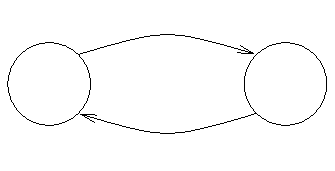
\includegraphics{figures/updown-automaton}%
\end{picture}%
\setlength{\unitlength}{4144sp}%
%
\begingroup\makeatletter\ifx\SetFigFont\undefined%
\gdef\SetFigFont#1#2{%
  \fontsize{#1}{#2pt}%
  \selectfont}%
\fi\endgroup%
\begin{picture}(2550,1296)(976,-1174)
\put(3151,-556){\makebox(0,0)[b]{\smash{{\SetFigFont{12}{14.4}{\color[rgb]{0,0,0}Down}%
}}}}
\put(3511,-556){\makebox(0,0)[lb]{\smash{{\SetFigFont{12}{14.4}{\color[rgb]{0,0,0}\lstinline{x = last x - 1}}%
}}}}
\put(1351,-556){\makebox(0,0)[b]{\smash{{\SetFigFont{12}{14.4}{\color[rgb]{0,0,0}Up}%
}}}}
\put(991,-556){\makebox(0,0)[rb]{\smash{{\SetFigFont{12}{14.4}{\color[rgb]{0,0,0}\lstinline{x = last x + 1}}%
}}}}
\put(2251,-61){\makebox(0,0)[b]{\smash{{\SetFigFont{12}{14.4}{\color[rgb]{0,0,0}$\mathtt{x} \geq 10$}%
}}}}
\put(2251,-1096){\makebox(0,0)[b]{\smash{{\SetFigFont{12}{14.4}{\color[rgb]{0,0,0}$\mathtt{x} \leq 0$}%
}}}}
\end{picture}%

  \caption{Automaton of the \texttt{updown} node}
  \label{fig:updown-automaton}
\end{figure}

\begin{lstlisting}
node updown() returns (y:int)
  var last x:int = 0;
let
  y = x;
  automaton
    state Up
      do x = last x + 1
      until x >= 10 then Down
    state Down
      do x = last x - 1
      until x <= 0 then Up
  end
tel
\end{lstlisting}

\[
\begin{streams}{9}
\text{current state} & Up & Up & \ldots & Up & Up & Down & Down & Down & \ldots\\\hline
\mathtt{y} & 1 & 2 & \ldots & 9 & 10 & 9 & 8 & 7 & \ldots\\\hline
\end{streams}
\]

 Expressions on outgoing transitions of this active state are
evaluated, so as to compute the next active state : these are weak
transitions. Transitions are evaluated in declaration order, in the textual
syntax. If no transition can be triggered, then the current state is the next
active state.

\paragraph{Weak and strong transitions.}

Transitions between states can be of two types: weak transitions, and strong
ones.

\subparagraph{Weak transitions} are denoted $\Until e \Then S$. The meaning of
such transition is that when $e$ becomes true, the current state is executed
before leaving it. The target state is only executed at next instant.

\subparagraph{Strong transitions} are denoted $\Unless e \Then S$. When $e$
becomes true, the automaton instantly leaves the current state, and the target
state is executed.

For causality reasons, the condition on strong transitions cannot depend
instantly on the variables defined in the current state (as this state is not
known and can change because of these transitions). Therefore, the example of
the Figure~\ref{fig:updown-automaton} can be written as shown below:

\begin{lstlisting}
node updown() returns (y:int)
  var last x:int = 0;
let
  y = x;
  automaton
    state Up
      do x = last x + 1
      unless (last x >= 10) then Down
    state Down
      do x = last x - 1
      unless (last x <= 0) then Up
  end
tel
\end{lstlisting}

On this example, the sequence of states is exactly the same as in the previous
version; however, the transition from $Up$ to $Down$ is taken one instant after
(i.e., the instant next to the one where $x=10$). The resulting stream
$\mathtt{y}$ is the same: 

\[
\begin{streams}{9}
\text{current state} & Up & Up & \ldots & Up & Up & Down & Down & Down & \ldots\\\hline
\mathtt{y} & 1 & 2 & \ldots & 9 & 10 & 9 & 8 & 7 & \ldots\\\hline
\end{streams}
\]

\paragraph{Transition and memory.}
When a transition (either weak or strong) denoted with \Then is taken, the
target state is reset in its initial state: such transitions are said
\emph{memoryless}. Conversely, \emph{transitions with memory} are denoted
$\Until e \Continue S$ (resp. $\Unless e \Continue S$): in that case, the target
state $S$ is executed without reset.

\subsection{Structured types}

\subsubsection{Arrays}

Arrays are denoted using the \lstinline+^+ symbol. For instance, \lstinline+int^10+ is the type of arrays of size 10 containing integers. Arrays can be multidimensional, like \lstinline{int^3^2}. One should note that indices appear in reverse order compared to C: \lstinline{int^3^2} should be understood as \lstinline{(int^3)^2}, that is an array of size 2 containing arrays of size 3 (this would have been written \lstinline{int t[2][3]} in C). \\

The following operators are defined for arrays:
\begin{itemize}
\item Accessing an element at a constant index: \lstinline{t[4]}
\item Accessing an element at a dynamic index with a default value: \lstinline{z = t.[x] default v} is a stream defined by $z_i = t_i[x_i]$ if $0 \leq x_i < n$ and $z_i = v_i$ otherwise (where $n$ is the size of \lstinline+t+).
\item Accessing an element at a truncated index: \lstinline+z = t[>x<]+ is defined by $z_i = t_i[\min(\max(0, x_i), n-1)]$ (where $n$ is the size of \lstinline+t+).
\item Modifying an element: \lstinline{t' = [ t with [x] = v ]} is a new array equal to \lstinline+t+, except for the element at index \lstinline+x+ which is equal to $v$, that is for all j in $[0, n-1]$ such that $j \neq x_i$, $t'_i[j] = t_i[j]$ and $t'_i[x_i] = v_i$.
\item Defining an array by copying one value: \lstinline+x^n+ is the array of size \lstinline+n+ whose elements are all equal to \lstinline+x+.
\item Defining an array explicitely:  \lstinline+[1, x, 3, y, 5]+.
\item Extracting a slice: \lstinline+t[n..m]+ returns the sub array of \lstinline+t+ of size \lstinline{m-n+1} starting at index \lstinline+n+ and ending at index \lstinline+m+.
\item Concatening arrays: \lstinline+t1@t2+.
\end{itemize}

It is also possible to use \emph{iterators} to operate on arrays. For instance, one can add two arrays pointwise by doing \lstinline{t = map<<n>> (+)(t1, t2)} (where \lstinline+n+ is the size of \lstinline+t1+, \lstinline+t2+ and \lstinline+t+).  The following iterators are defined:
\begin{itemize}
\item \lstinline+map+ applies a node pointwise to the input arrays and outputs one or several arrays. If \lstinline+f+ has type \lstinline+t1 * t2 -> t'1 * t'2+ then \lstinline+map<<n>> f+ has type \lstinline+t1^n * t2^n -> t'1^n * t'2^n+.
\item \lstinline+mapi+ is the same as \lstinline+map+ but the iterated function should expect another integer argument, which will be equal to the index of the inputs in the input arrays. If \lstinline+f+ has type \lstinline+t1 * t2 * int -> t'1 * t'2+ then \lstinline+map<<n>> f+ has type \lstinline+t1^n * t2^n -> t'1^n * t'2^n+. 
\item \lstinline+fold+ iterates a node on an array accumulating values. If \lstinline+f+ has type \lstinline+t1 * t -> t+ then \lstinline+fold<<n>> f+ has type \lstinline+t1^n * t -> t+. For instance,  \lstinline+fold<<2>> f(t, 0)+ is equivalent to  \lstinline+f(t[1], f(t[0], 0))+.
\item \lstinline+foldi+ is to  \lstinline+fold+ what  \lstinline+mapi+ is to  \lstinline+map+.
\item  \lstinline+mapfold+ combines the result of  \lstinline+map+ and  \lstinline+fold+, by accumulating a value and outputting a new array. If \lstinline+f+ has type \lstinline+t1 * t -> t'1 * t+ then \lstinline+mapfold<<n>> f+ has type \lstinline+t1^n * t -> t'1^n * t+.
\end{itemize}

\begin{figure}[htp]
 \centering
 \subfigure[\texttt{map}]{
 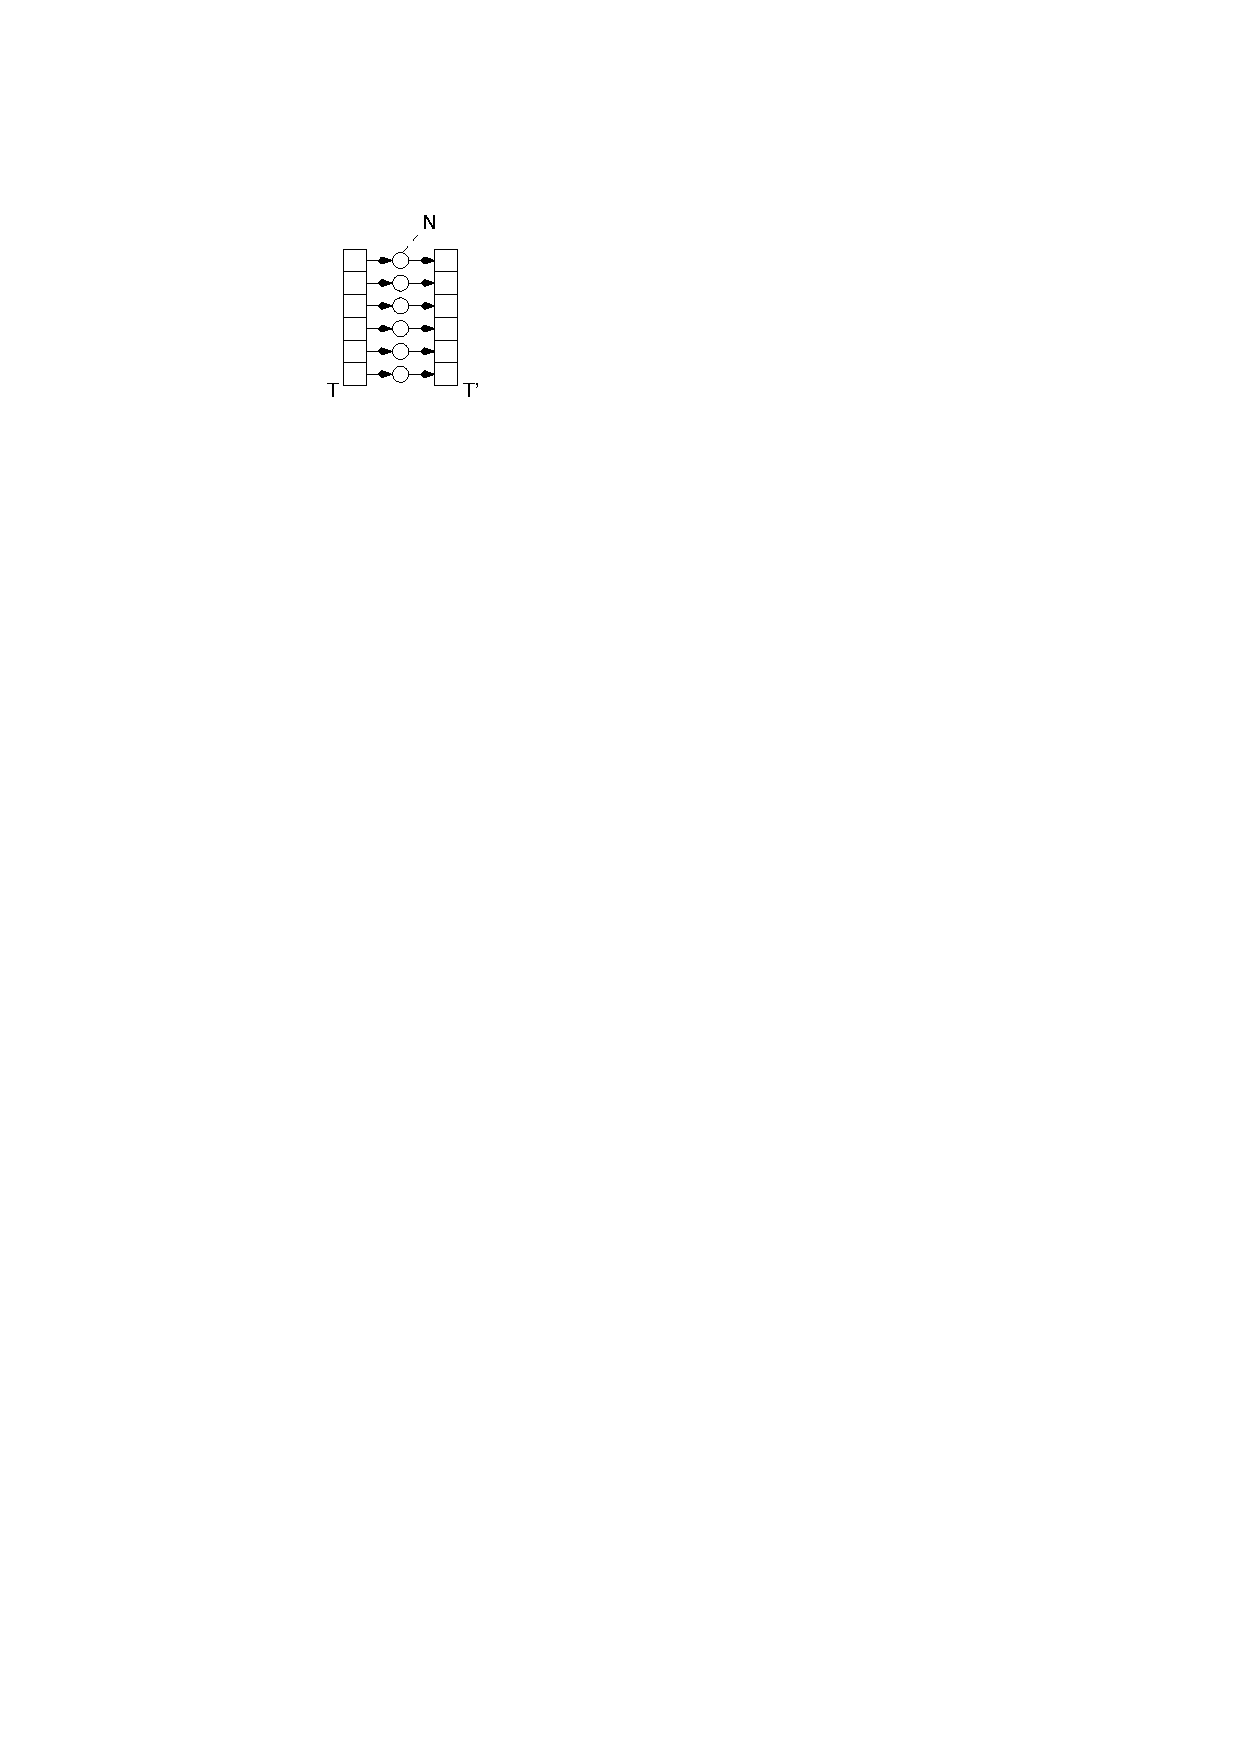
\includegraphics[width = 0.25\textwidth]{figures/map}
  }
 \subfigure[\texttt{fold}]{
  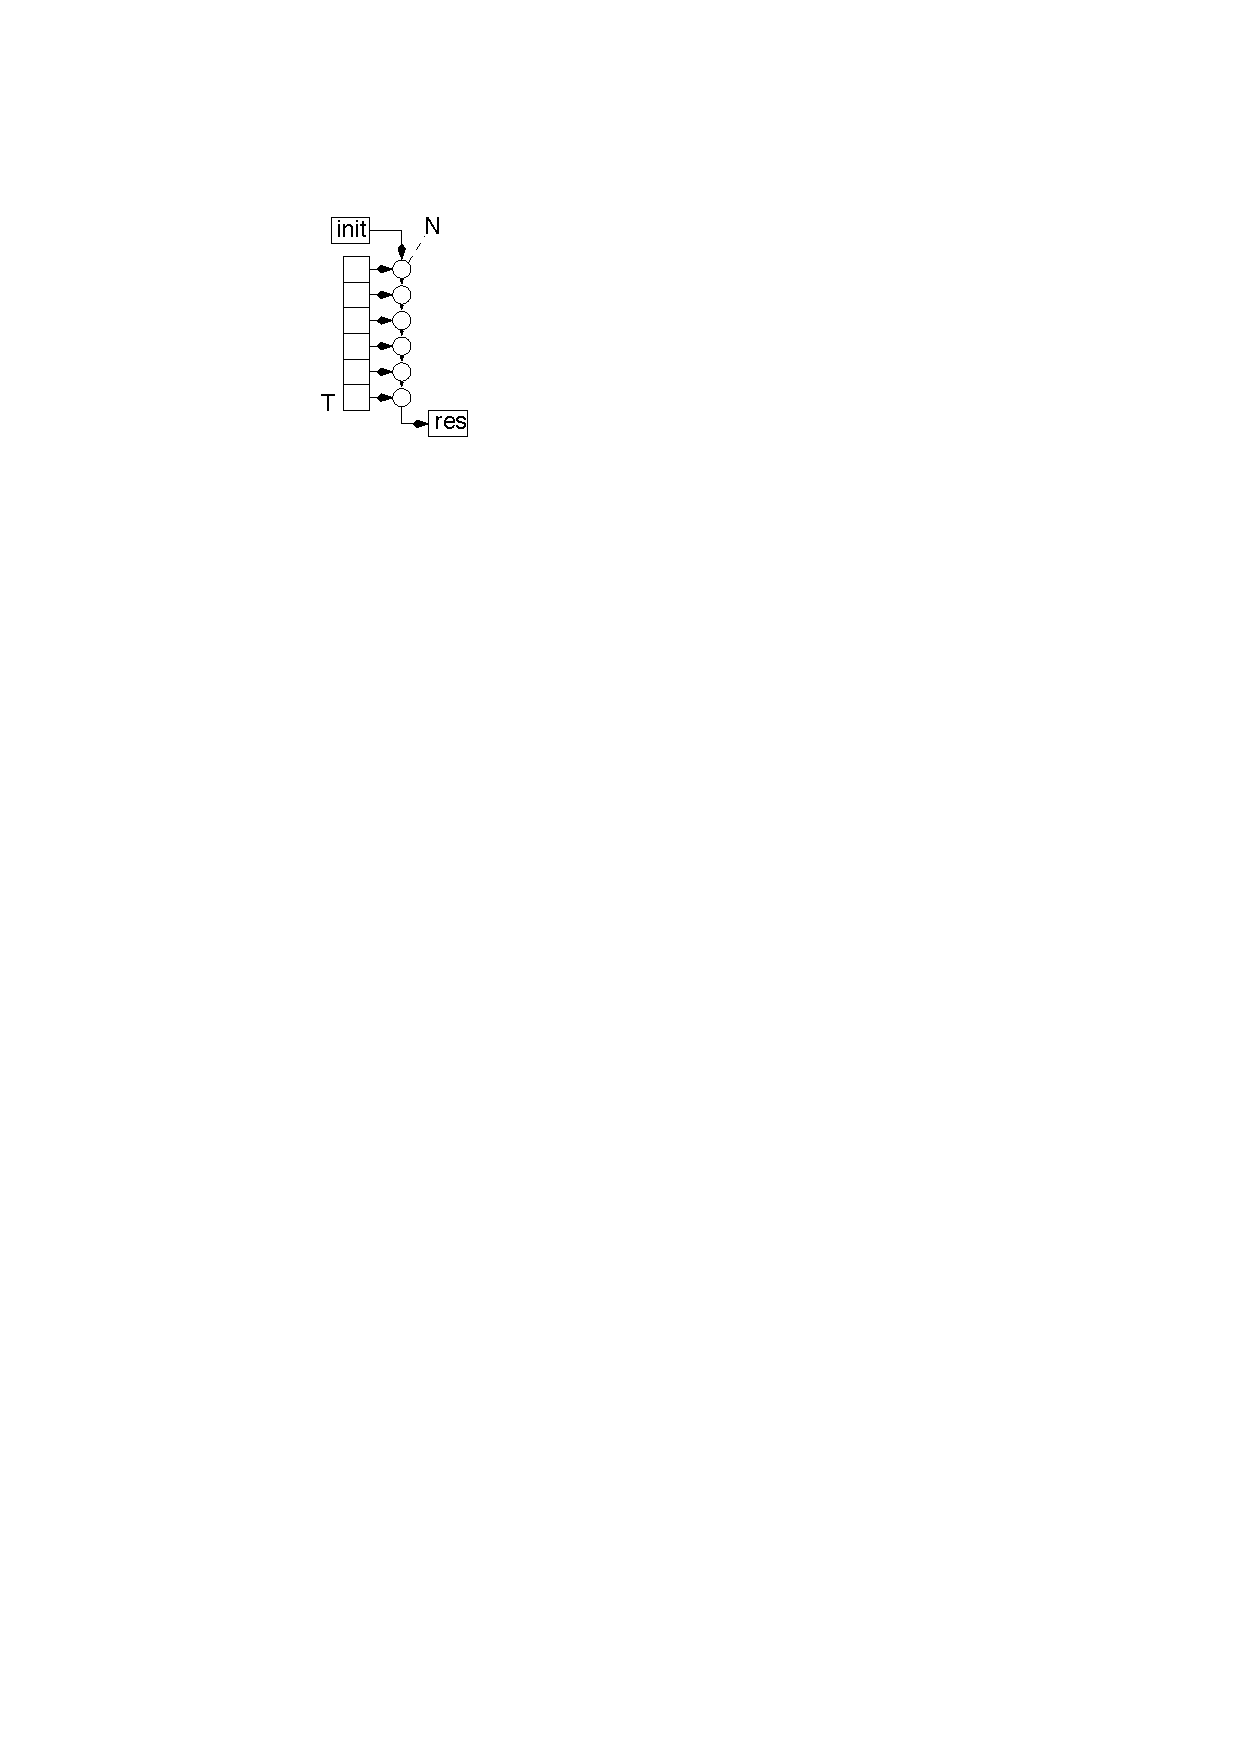
\includegraphics[width = 0.25\textwidth]{figures/fold}
  }
 \subfigure[\texttt{mapfold}]{
  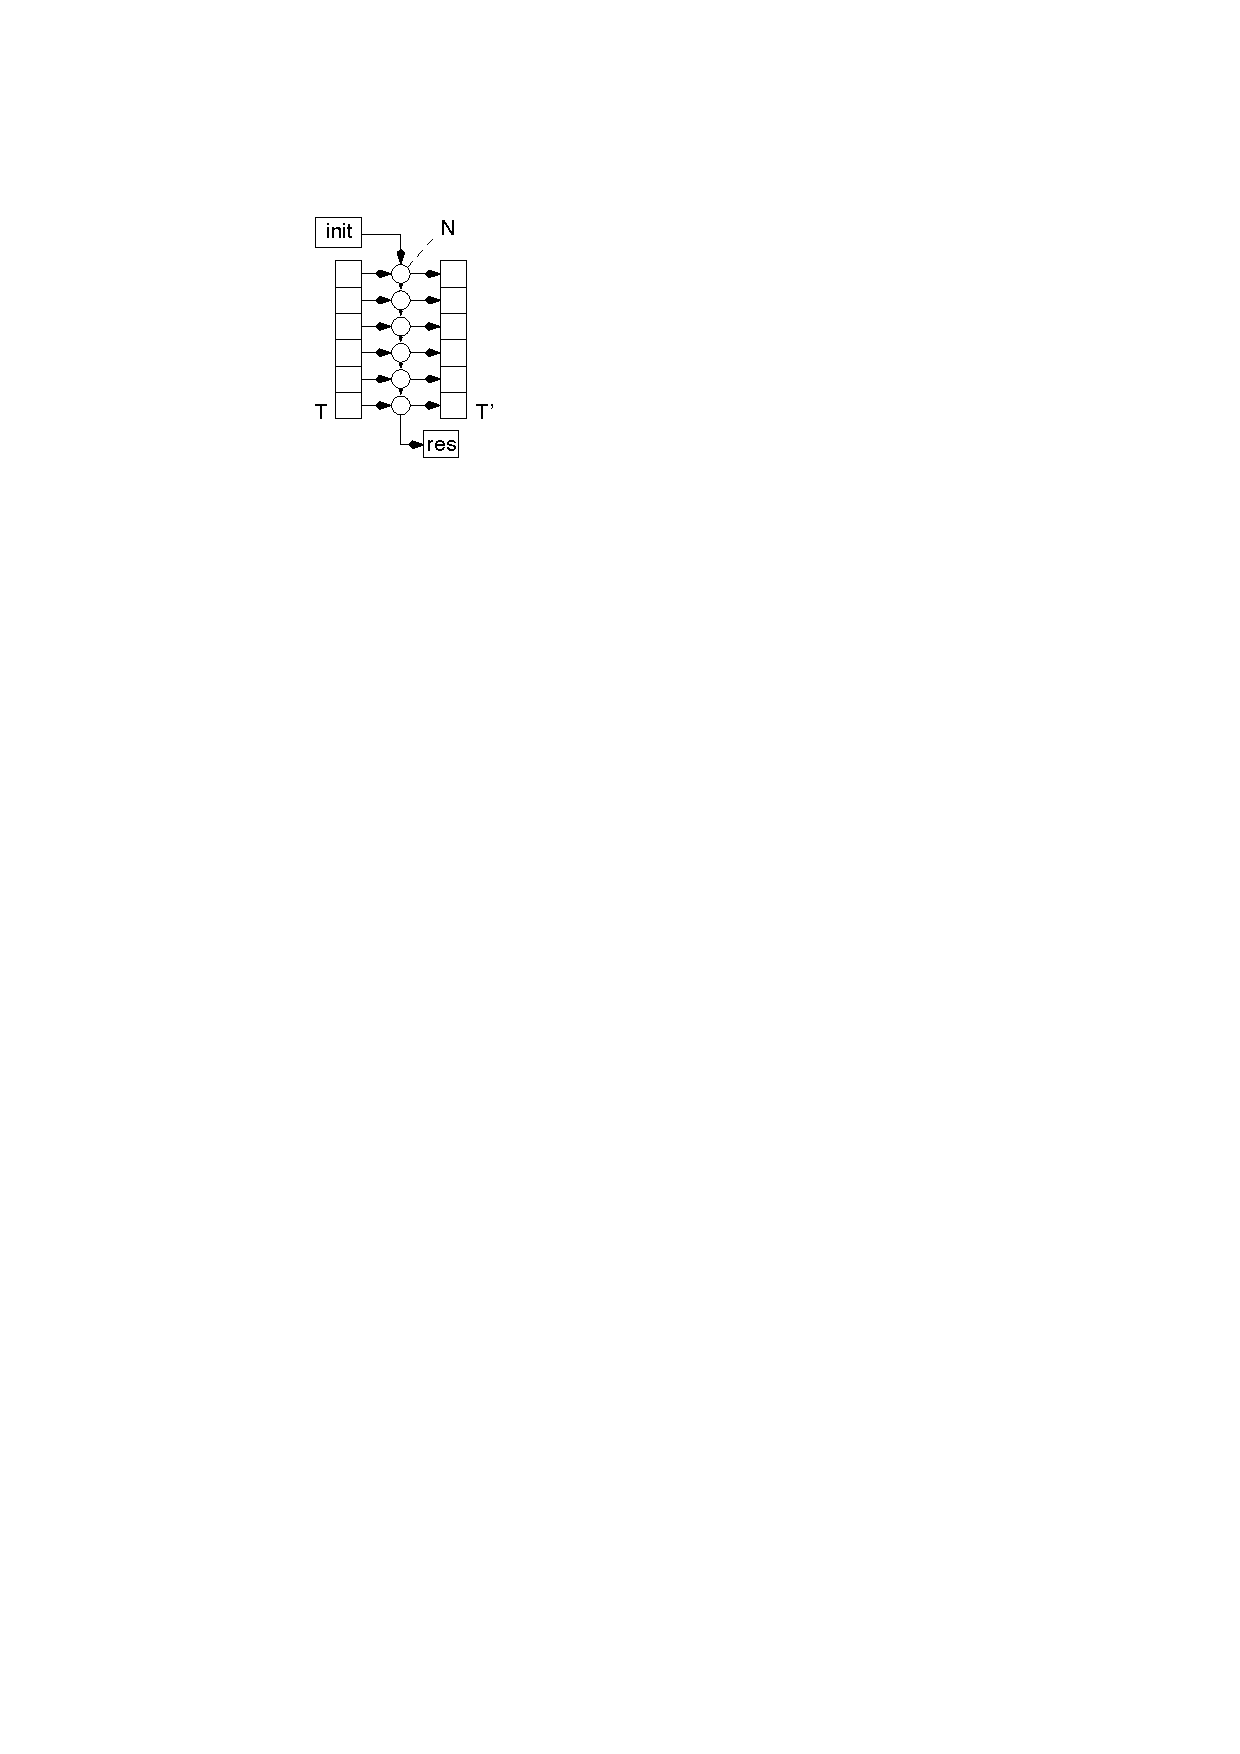
\includegraphics[width = 0.25\textwidth]{figures/mapfold}
  }
  \caption{Iterators in \textsc{Heptagon}}
  \label{fig:iterators}
\end{figure}

Iterators can also be used for multidimensional arrays. In the case of \lstinline+mapi+ and \lstinline+foldi+, the iterated function should then expect one argument for each dimension.

It is also possible to mimic partial application with iterators, by giving a list of arguments, not necessarily arrays, that will be given as first arguments to each application of the iterated function. For instance, \lstinline+o = map<<n>>f <(a)>(t)+ is equivalent to \lstinline+o[i] = f(a, t[i])+ for each element in the output array \lstinline+o+.

Arrays are semantically functional: each modification on an array creates a new array. Implementing these arrays using separate arrays can lead to very unefficient code. That's why an optimization pass called \emph{memory allocation}~\cite{Gerard:2012} tries to share arrays and avoid unnecessary copies within each node. It can be enabled using the \texttt{-memalloc} or \texttt{-O} option.

\subsubsection{Records}

The syntax for declaring record types is the following:
\begin{lstlisting}
type t = { f1: t1; f2: t2 }
\end{lstlisting}
Note that two different record types cannot have fields with the same name.
It is possible to declare a new record (\lstinline+{ f1 = x; f2 = 9 }+), read a field of a record (\lstinline+x.f1+) and modify one field (\lstinline+r' = { r with .f1 = v }+ returns a new record where all fields are equal to the ones in \lstinline+r+ except for \lstinline+f1+ which is equal to \lstinline+v+). 

\subsubsection{Types alias}

It is possible to declare an alias for any type (like a \texttt{typedef} in C), for instance:
\begin{lstlisting}
type meter = int
type matrix = int^10^10
\end{lstlisting}
This alias can then be used anywhere a type is expected.


\subsection{Parametricity}

The size of arrays can be parametrized by so-called \emph{static expressions}, that is expressions that are reduced to constants at compile-time. They are either a literal, a global constant, a static parameter of a node or a static operation on two static expressions (\lstinline{+}, \lstinline{-}, \lstinline{*}, \lstinline{/}, \lstinline{+.}, \lstinline{<=}, \lstinline{or}, etc). Global constants are declared by:
\begin{lstlisting}
const n : int = 100
const t0 : float^n = 1.0^n
const r0 = { f1 = 0; f2 = t0 }
\end{lstlisting}

The parameters of a node are given between \lstinline+<<+ and \lstinline{>>} at the declaration of the node and are instantiated with the same syntax:
\begin{lstlisting}
node f<<m:int; t1: int^n>>(a:int^m) = (o:int^m)
let
  o = map<<m>> (+)(a, t1);
tel

node g(a:int^n) = (o:int^n)
let
  o = f<<n, t0>>(a);
tel
\end{lstlisting}

If the backend support parametricity (like in Java), static parameters are kept in the generated code. Otherwise, a pass of the compiler generates all the versions of the node that are needed. If a parametrized node defined in a file \texttt{f1.ept} is used in \texttt{f2.ept}, it is necessary to first compile \texttt{f1.ept} with the \texttt{-c} option (and without any \texttt{-target}), in order to generate a binary file \texttt{f1.epo}. The compilation of the second file, this time with the \texttt{-target} option, will generate code for all the necessary nodes, from \texttt{f1.ept} and \texttt{f2.ept}.

\subsection{Location annotations}

Memory allocation~\cite{Gerard:2012} avoids unnecessary array copies within the nodes automatically (it can be enable with the \texttt{-memalloc} or \texttt{-O} options). In order to avoid copies when calling nodes, the user must add \emph{location annotations}. We will give here only a short introduction, the interested reader can refer to~\cite{Gerard:2012} for more details. They express the fact that a function modifies in-place its argument. For instance, consider this node that swaps two elements in an array:
\begin{lstlisting}
node swap(i, j:int; t_in:float^100 at r) returns (t_out:float^100 at r)
var t_tmp:float^100 at r; 
let
  t_tmp = [ t_in with [i] = t_in[>j<] ]; 
  t_out = [ t_tmp with [j] = t_in[>i<] ];
tel
\end{lstlisting}
The location annotations are introduced by the keyword \lstinline{at} followed by a location name. All the streams with the same location name are guaranteed to be stored together in the generated code, so the function generated for \texttt{swap} will directly modify its argument in-place. 

Located variables are called \emph{semilinear}: they can only be updated once, but they can be read many times. An update is a function that modify its argument in-place, for instance a node that inputs and outputs located variables, and a read is any other function. For instance, modifying one element in an array is an update, but accessing one element is a read.

Only located variables can be given to a function that expects located arguments. A located variable can only be obtained by updating another located variable or by explicitly initializing a new location with the \lstinline+init+ construction:
\begin{lstlisting}
node shuffle(i_arr, j_arr : int^m; q : int) = (v : float)
var t, t_prev : float^n at r;
let
  init<<r>> t_prev = t_0 fby t;
  t = fold<<m>> swap(i_arr, j_arr, t_prev); 
  v = t[>q<];
tel
\end{lstlisting}


\subsection{Interfaces}

Interface files, with the extension \texttt{.epi}, do not contain any definition but only the declaration (or signatures) of nodes, types and constants. In particular, they are useful to import external functions. For instance:
\begin{lstlisting}
external fun sort(a:int^100) = (o:int^100)
\end{lstlisting}
The imported function should respect the calling convention given in appendix \ref{sec:app-generated-code}. See the directory \texttt{examples/extern\_C} for a complete example.

Interface files can be compiled with \texttt{heptc}, in order to obtain a
compiled interface (\texttt{.epci} file), necessary for the subsequent use of
the declared types and values in other Heptagon programs.

\subsection{Contracts for controller synthesis}
\label{sec:extens-with-contr}

Contracts are an extension of the Heptagon language, so as to allow to perform
discrete controller synthesis (DCS) on Heptagon programs. The extended language is
named BZR.

We associate to each node a \emph{contract}, which is a program associated with
two outputs :
\begin{itemize}
\item an output $e_A$ representing the environment model ;
\item an invariance objective $e_G$ ;
\item a set $\set{\ton{c}{,}}$ of controllable variables used for ensuring this objective.
\end{itemize}

This contract means that the node will be controlled, i.e., that values will be
given to $\ton{c}{,}$ such that, given any input trace yielding $e_A$, the
output trace will yield the true value for $e_G$.

Contracts are denoted :
\begin{lstlisting}
node f(x$_1$:t$_1$;$\ldots$;x$_n$:t$_n$) returns (y$_1$:t$'_1$;$\ldots$;y$_p$:t$'_p$)
contract
  var $\ldots$
  let
     $\ldots$
  tel
  assume $e_A$
  enforce $e_G$
  with (c$_1$:t$''_1$;$\ldots$;c$_q$:t$''_n$)

var $\ldots$
let
  y$_1$ = f$_1$($\ton{\mathtt{x}}{,},\ton[1][q]{\mathtt{c}}{,}$); 
  $\vdots$
  y$_p$ = f$_p$($\ton{\mathtt{x}}{,},\ton[1][q]{\mathtt{c}}{,}$); 
tel
\end{lstlisting}

\section{Example with Contracts:  Multi-task System}
\label{sec:multi-task-system}

\subsection{Delayable Tasks}
\label{sec:delayable-tasks}



We consider a multi-task system composed of $n$ delayable
tasks. Figure~\ref{fig:del-task} shows a delayable task. A delayable task takes
three inputs \texttt{r}, \texttt{c} and \texttt{e}: \texttt{r} is the task
launch request from the environment, \texttt{e} is the end request, and
\texttt{c} is meant to be a controllable input controlling whether, on request,
the task is actually launched (and therefore goes in the active state), or
delayed (and then forced by the controller to go in the waiting state by stating
the false value to \texttt{c}). This node outputs a unique boolean \texttt{act}
which is true when the task is in the active state.

\begin{figure}[htb]
\begin{lstlisting}
node delayable(r,c,e:bool) returns (act:bool)
  let
    automaton
      state Idle
        do act = false
        until r & c then Active
            | a & not c then Wait
      state Wait
        do act = false
        until c then Active
      state Active
        do act = true
        until e then Idle
    end
  tel
\end{lstlisting}
\caption{Delayable task}
\label{fig:del-task}
\end{figure}

The Figure~\ref{fig:n-del-task} shows then a node \texttt{ntasks} where $n$
delayable tasks have been put in parallel. The tasks are inlined so as to be
able to perform DCS on this node, taking into account the tasks' states. Until
now, the only interest of modularity is, from the programmer's point of view, to
be able to give once the delayable task code.

\begin{figure}[htb]
\begin{lstlisting}
node ntasks($\ton{\mathtt{r}}{,},\ton{\mathtt{e}}{,}$:bool)
       returns ($\ton{\mathtt{a}}{,}$:bool)
  contract
  let
    ca$_{1}$ = a$_{1}$ & (a$_{2}$ or $\ldots$ or a$_{n}$);
    $\vdots$
    ca$_{n-1}$ = a$_{n-1}$ & a$_{n}$;
  tel
  enforce not (ca$_{1}$ or \ldots or ca$_{n-1}$) 
  with ($\ton{\mathtt{c}}{,}$:bool)
let
  a$_{1}$ = inlined delayable(r$_{1}$,c$_{1}$,e$_{1}$); 
  $\vdots$
  a$_{n}$ = inlined delayable(r$_{n}$,c$_{n}$,e$_{n}$); 
tel
\end{lstlisting}
\caption{\texttt{ntasks} node: $n$ delayable tasks in parallel}
\label{fig:n-del-task}
\end{figure}

This \texttt{ntasks} node is provided with a contract, stating that its
composing tasks are exclusive, i.e., that there are no two tasks in the active
state at the same instant. This contract is enforced with the help of the
controllable inputs $c_i$.

\subsection{Contract composition}
\label{sec:contract-composition}

We want know to reuse the \texttt{ntasks} node, in order to build modularly a
system composed of $2n$ tasks. The Figure~\ref{fig:2n-del-task} shows the
parallel composition of two \texttt{ntasks} nodes. We associate to this
composition a new contract, which role is to enforce the exclusivity of the $2n$
tasks.

\begin{figure}[htb]
\begin{lstlisting}
node main($\ton[1][2n]{\mathtt{r}}{,},\ton[1][2n]{\mathtt{e}}{,}$:bool)
       returns ($\ton[1][2n]{\mathtt{a}}{,}$:bool)
  contract
  let
    ca$_{1}$ = a$_{1}$ & (a$_{2}$ or $\ldots$ or a$_{2n}$);
    $\vdots$
    ca$_{2n-1}$ = a$_{2n-1}$ & a$_{2n}$;
  tel
  enforce not (ca$_{1}$ or $\ldots$ or ca$_{2n-1}$)
let
  ($\ton{\mathtt{a}}{,}$) = ntasks($\ton{\mathtt{r}}{,}$,$\ton{\mathtt{e}}{,}$); 
  ($\ton[n+1][2n]{\mathtt{a}}{,}$) = ntasks($\ton[n+1][2n]{\mathtt{r}}{,}$,$\ton[n+1][2n]{\mathtt{e}}{,}$); 
tel
\end{lstlisting}
\caption{Composition of two \texttt{ntasks} nodes}
\label{fig:2n-del-task}
\end{figure}

It is easy to see that the contract of \texttt{ntasks} is not precise enough to
be able to compose several of these nodes. Therefore, we need to refine this
contract by adding some way to externally control the activity of the tasks.

\subsection{Contract refinement}
\label{sec:contract-refinement}

We first add an input \texttt{c}, meant to be controllable. The refined contract
will enforce that:
\begin{enumerate}
\item the tasks are exclusive,
\item one task is active only at instants when the input \texttt{c} is
  true. This property, appearing in the contract, allow a node instantiating
  \texttt{ntasks} to forbid any activity of the $n$ tasks instantiated.
\end{enumerate}
The Figure~\ref{fig:n-del-task-2} contains this new \texttt{ntasks} node.

\begin{figure}[htb]
\begin{lstlisting}
node ntasks(c,$\ton{\mathtt{r}}{,}$,$\ton{\mathtt{e}}{,}$:bool) returns ($\ton{\mathtt{a}}{,}$:bool)
  contract
  let
    ca$_{1}$ = a$_{1}$ & (a$_{2}$ or $\ldots$ or a$_{n}$);$\ldots$
    ca$_{n-1}$ = a$_{n-1}$ & a$_{n}$;
    one = a$_{1}$ or $\ldots$ or a$_{n}$;
  tel
  enforce not (ca$_{1}$ or $\ldots$ or ca$_{n-1}$) & (c or not one)
  with ($\ton{\mathtt{c}}{,}$:bool)
let
  a$_{1}$ = inlined delayable(r$_{1}$,c$_{1}$,e$_{1}$); 
  $\vdots$
  a$_{n}$ = inlined delayable(r$_{n}$,c$_{n}$,e$_{n}$); 
tel
\end{lstlisting}
\caption{First contract refinement for the \texttt{ntasks} node}
\label{fig:n-del-task-2}
\end{figure}

\begin{figure}[htb]
  \centering
\begin{lstlisting}
node ntasks(c,$\ton{\mathtt{r}}{,}$,$\ton{\mathtt{e}}{,}$:bool) returns ($\ton{\mathtt{a}}{,}$:bool)
  contract
  let
    ca$_{1}$ = a$_{1}$ & (a$_{2}$ or $\ldots$ or a$_{n}$);$\ldots$
    ca$_{n-1}$ = a$_{n-1}$ & a$_{n}$;
    one =  a$_{1}$ or $\ldots$ or a$_{n}$;
    pone = false fby one;
  tel
  assume (not pone or c)
  enforce not (ca$_{1}$ or $\ldots$ or ca$_{n-1}$) & (c or not one)
  with ($\ton{\mathtt{c}}{,}$)
let
  a$_{1}$ = inlined delayable(r$_{1}$,c$_{1}$,e$_{1}$); 
  $\vdots$
  a$_{n}$ = inlined delayable(r$_{n}$,c$_{n}$,e$_{n}$); 
tel
\end{lstlisting}
  \caption{Second contract refinement for the \texttt{ntasks} node}
  \label{fig:n-del-tasks-3}
\end{figure}

However, the controllability introduced here is know too strong. The synthesis
will succeed, but the computed controller, without knowing how \texttt{c} will
be instantiated, will actually block every tasks in their idle state. Indeed, if
the controller allows one task to go in its active state, the input \texttt{c}
can become false at the next instant, violating the property to enforce.

Thus, we propose to add an assumption to this contract: the input \texttt{c}
will not become false if a task was active an instant before. This new contract
is visible in Figure~\ref{fig:n-del-tasks-3}.

We can then use this new \texttt{ntasks} version for the parallel composition,
by instantiating the \texttt{c} input by a controllable variable and its
negation. This composition can be found in Figure~\ref{fig:ntasks-compos}.

\begin{figure}[htb]
  \centering
\begin{lstlisting}
node main($\ton[1][2n]{\mathtt{r}}{,}$,$\ton[1][2n]{\mathtt{e}}{,}$:bool) returns ($\ton[1][2n]{\mathtt{a}}{,}$:bool)
  contract
  let
    ca$_{1}$ = a$_{1}$ & (a$_{2}$ or $\ldots$ or a$_{2n}$);
    $\vdots$
    ca$_{2n-1}$ = a$_{2n-1}$ & a$_{2n}$;
  tel
  enforce not (ca$_{1}$ or $\ldots$ or ca$_{2n-1}$)
  with (c:bool)
let
  ($\ton{\mathtt{a}}{,}$) = ntasks(c,$\ton{\mathtt{r}}{,}$,$\ton{\mathtt{e}}{,}$); 
  ($\ton[n+1][2n]{\mathtt{a}}{,}$) = ntasks(\Not c,$\ton[n+1][2n]{\mathtt{r}}{,}$,$\ton[n+1][2n]{\mathtt{e}}{,}$); 
tel
\end{lstlisting}
  \caption{Two \texttt{ntasks} parallel composition}
  \label{fig:ntasks-compos}
\end{figure}

\section{Known issues}
\label{sec:known-issues}

Heptagon is a research prototype. Users are kindly invited to submit bugs to the
Heptagon developers via \url{heptagon-developers@lists.gforge.inria.fr}

Yet, the following subject are known to be issues for the current Heptagon
version:
\begin{itemize}
\item Discrete controller synthesis (DCS) can be applied only on full Boolean
  programs (with static integer expressions). If applied on nodes containing
  non-Boolean expressions or values, an abstraction will be computed, removing
  every equation containing untranslatable value or expression. This abstraction
  is conservative w.r.t. invariance properties, and does not jeopardize the use
  of the computed controller, but this controller itself can be less efficient
  due to the abstraction.
\item For the above reason, DCS does not mix well with array types, which will
  be abstracted.
\item Translation to \texttt{Sigali} code (\texttt{-target z3z} option) for DCS
  application activates the \texttt{-bool} option, for translation of enumerated
  values into Boolean vectors. This translation cannot be applied on nodes whose
  signature comprise enumerated clocks, e.g., the node \lstinline{filter} below:

\begin{lstlisting}
type t = A | B

node filter(x:int; c:t) returns (y:int on A(c))
let
  y = x when A(c)
tel
\end{lstlisting}

\item Nodes whose signature comprise sampled streams cannot be inlined. However,
  inlining of nodes comprising clocks without appearing in signature is
  possible.
\end{itemize}

\clearpage
\appendix

\section{Generated code}
\label{sec:app-generated-code}

\subsection{C generated code}
\label{sec:c-generated-code}

C generated files from an Heptagon program \texttt{example.ept} are placed in a
directory named \texttt{example\_c}. This directory contains one file
\texttt{example.c}. For each node \texttt{f} of the source program, assuming
that \texttt{f} has inputs $(x_1:t_1,\ldots,x_n:t_n)$ and outputs
$(y_1:t'_1,\ldots,y_p:t'_p)$, $t_i$ and $t'_i$ being the data types of these
inputs and outputs, then the \texttt{example.c} file contains, for each node
\texttt{f}:

\begin{itemize}
\item A \texttt{Example\_\_f\_reset} function, with an argument \texttt{self} being a
  memory structure instance:

\begin{lstlisting}[language=C]
void Example__f_reset(Example__f_mem* self);
\end{lstlisting}

\item A \texttt{Example\_\_f\_step} function, with as arguments the nodes inputs, a
  structure \texttt{\_out} where the output will be put, and a memory structure
  instance \texttt{self}:

\begin{lstlisting}[language=C]
void Example__f_step(t$_{1}$ x$_{1}$, ..., t$_{n}$ x$_{n}$,
                     Example__f_out* \_out,
                     Example__f_mem* self);
\end{lstlisting}

After the call of this function, the structure \texttt{\_out} contains the
outputs of the node:
\begin{lstlisting}[language=C]
typedef struct \{
  t$'_1$ y$_{1}$;
  ...
  t$'_p$ y$_{p}$;
\} Example__f_out;
\end{lstlisting}
\end{itemize}

An example of main C code for the execution of this node would be then:
\begin{lstlisting}[language=C]
#include "example.h"

int main(int argc, char * argv[]) {
  
  Example__f_m mem;
  t$_{1}$ x$_{1}$;
  ...
  t$_{n}$ x$_{n}$;
  Example__f_out ans;

  /* initialize memory instance */
  f_reset(&mem);
  
  while(1) {
    /* read inputs */
    scanf("...", &x$_{1}$, ..., &x$_{n}$);

    /* perform step */
    Example__f_step(x$_{1}$, ..., x$_{n}$, &ans, &mem);

    /* write outputs */
    printf("...", ans.y$_{1}$, ..., ans.y$_{p}$);
  }
}
\end{lstlisting}

The above code is nearly what is produce for the simulator with the \texttt{-s}
option (see Section~\ref{sec:simulation}).

% \subsection{OCaml generated code}
% \label{sec:ocaml-generated-code}


% If the option \texttt{-target caml} is given, then the compiler generates OCaml
% code in a file named \texttt{example.ml}. Heptagon nodes are compiled into OCaml
% classes, where state variables are class properties, and the two functions
% ``reset'' and ``step'' are class methods. Thus, the class type of \texttt{f}
% would be:
% \begin{alltt}
% class f :
%   object
%     method reset : unit \(\rightarrow\) unit
%     method step : t\ind{1} * ... * t\ind{n} \(\rightarrow\) (t\('\sb{1}\) * ... * t\('\sb{p}\))
%   end
% \end{alltt}

\subsection{Java generated code (Java 1.5 and above)}
\label{sec:java-generated-code}

Java generated files from an Heptagon program \texttt{example.ept} are placed in
a directory named \texttt{java/Example}, constituted in a Java package named
\texttt{Example}. This directory contains one Java class \texttt{F} (in the file
\texttt{F.java}) for each node \texttt{f} of the source program. Assuming that
\texttt{f} has inputs $(x_1:t_1,\ldots,x_n:t_n)$ and outputs
$(y_1:t'_1,\ldots,y_p:t'_p)$, $t_i$ and $t'_i$ being the data types of these
inputs and outputs, then this \texttt{f} class implements the following
interface:


\begin{lstlisting}[language=Java]
public interface f {
    
    public void reset();

    public jeptagon.Pervasives.Tuple$n$ step(t$_{1}$ x$_{1}$, ..., t$_{n}$ x$_{n}$);
}
\end{lstlisting}

The \texttt{Tuple$n$} class is a $n$-uple (as a composite of $n$ \texttt{Object}
instances). The output $y_1\ldots y_n$ are accessible through the properties
\texttt{c0}\ldots\texttt{c$(n-1)$} of the \texttt{Tuple$n$}'s instance.

\subsection{Java generated code (Java 1.4)}
\label{sec:java14-generated-code}

The option \texttt{-target java14} generated Java 1.4 compliant code (typically,
without enumerated types and genericity).

Java generated files from an Heptagon program \texttt{example.ept} are placed in
a directory named \texttt{java/Example}, constituted in a Java package named
\texttt{Example}. This directory contains one Java class \texttt{F} (in the file
\texttt{F.java}) for each node \texttt{f} of the source program. Assuming that
\texttt{f} has inputs $(x_1:t_1,\ldots,x_n:t_n)$ and outputs
$(y_1:t'_1,\ldots,y_p:t'_p)$, $t_i$ and $t'_i$ being the data types of these
inputs and outputs, then this \texttt{f} class implements the following
interface:

\begin{lstlisting}[language=Java]
public interface f {
    
    public void reset();

    public void step(t$_{1}$ x$_{1}$, ..., t$_{n}$ x$_{n}$);

    public $\mathtt{t}'_1$ getOutput0();
    $\vdots$
}
\end{lstlisting}


\bibliographystyle{plain}
\bibliography{manual}


\end{document}
